
\documentclass[12pt]{article}
\usepackage[utf8]{inputenc}
\usepackage{graphicx}
\usepackage{float}
\usepackage{titlesec}
\usepackage{geometry}
\usepackage{caption}
\usepackage[colorlinks=true, linkcolor=blue]{hyperref}

\geometry{margin=1in}
\titleformat{\section}{\normalfont\Large\bfseries}{}{0em}{}

\title{Norman’s Principles Retrospective Evaluation – GenreGuru}
\date{}

\begin{document}

\begin{titlepage}
    \centering
    {\scshape\LARGE McMaster University \par}
    \vspace{1cm}
    {\scshape\Large SFWRENG 4G06 Capstone Project\par}
    \vspace{1.5cm}
    {\huge\bfseries Norman’s Principles Retrospective Evaluation\par}
    \vspace{0.5cm}
    {\Large\itshape GenreGuru\par}
    \vfill
    \textbf{Team:} Rhythm Rangers (Team 8) \\
    \textbf{Team Members:} Muhammad Jawad, Ansel Chen, Mohamad-Hassan Bahsoun, Ahmed Al-Hayali \\
    \vfill
    {\large \today\par}
\end{titlepage}


\section*{Introduction}
This document evaluates the user interface (UI) design of GenreGuru based on Norman’s Design Principles. Each principle is examined in terms of both positive and negative applications within the current version of the system. Our evaluation is grounded in real user interaction with the interface, demonstrated through screenshots and a walkthrough of the core flow: searching a song, previewing it, selecting it, and receiving recommendations.

\section*{Screenshots}
\begin{figure}[H]
    \centering
    
\includegraphics[width=\textwidth]{normans_principles_figures/img1.jpg}
    \caption{GenreGuru Home Page}
    \label{img1}
\end{figure}

\begin{figure}[H]
    \centering
    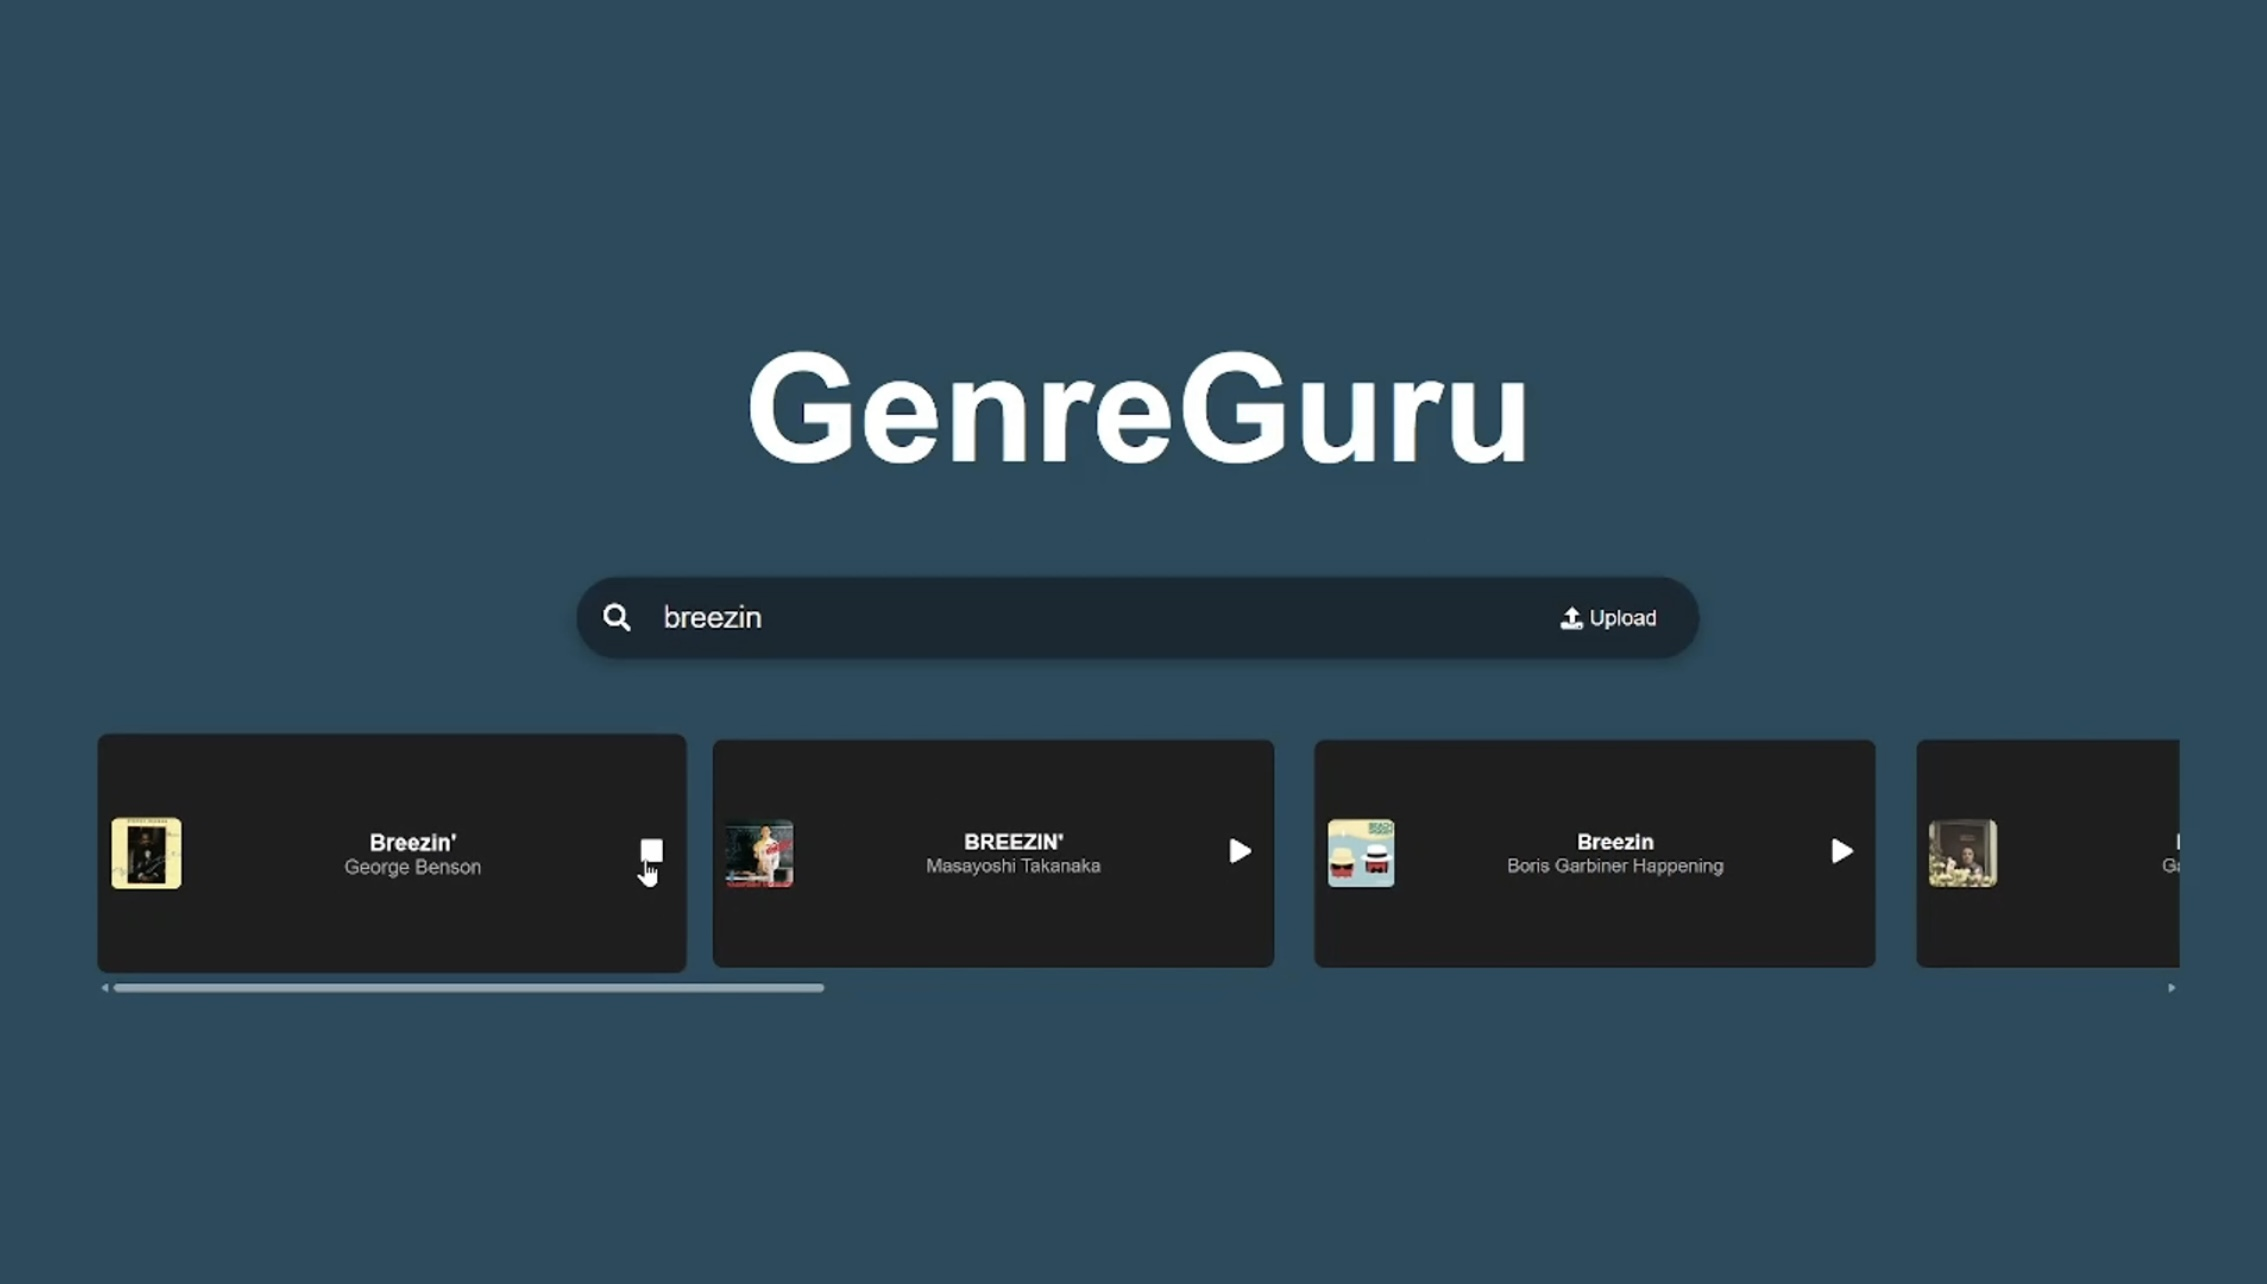
\includegraphics[width=\textwidth]{normans_principles_figures/img2.jpg}
    \caption{Search Results Page}
    \label{img2}
\end{figure}

\begin{figure}[H]
    \centering
    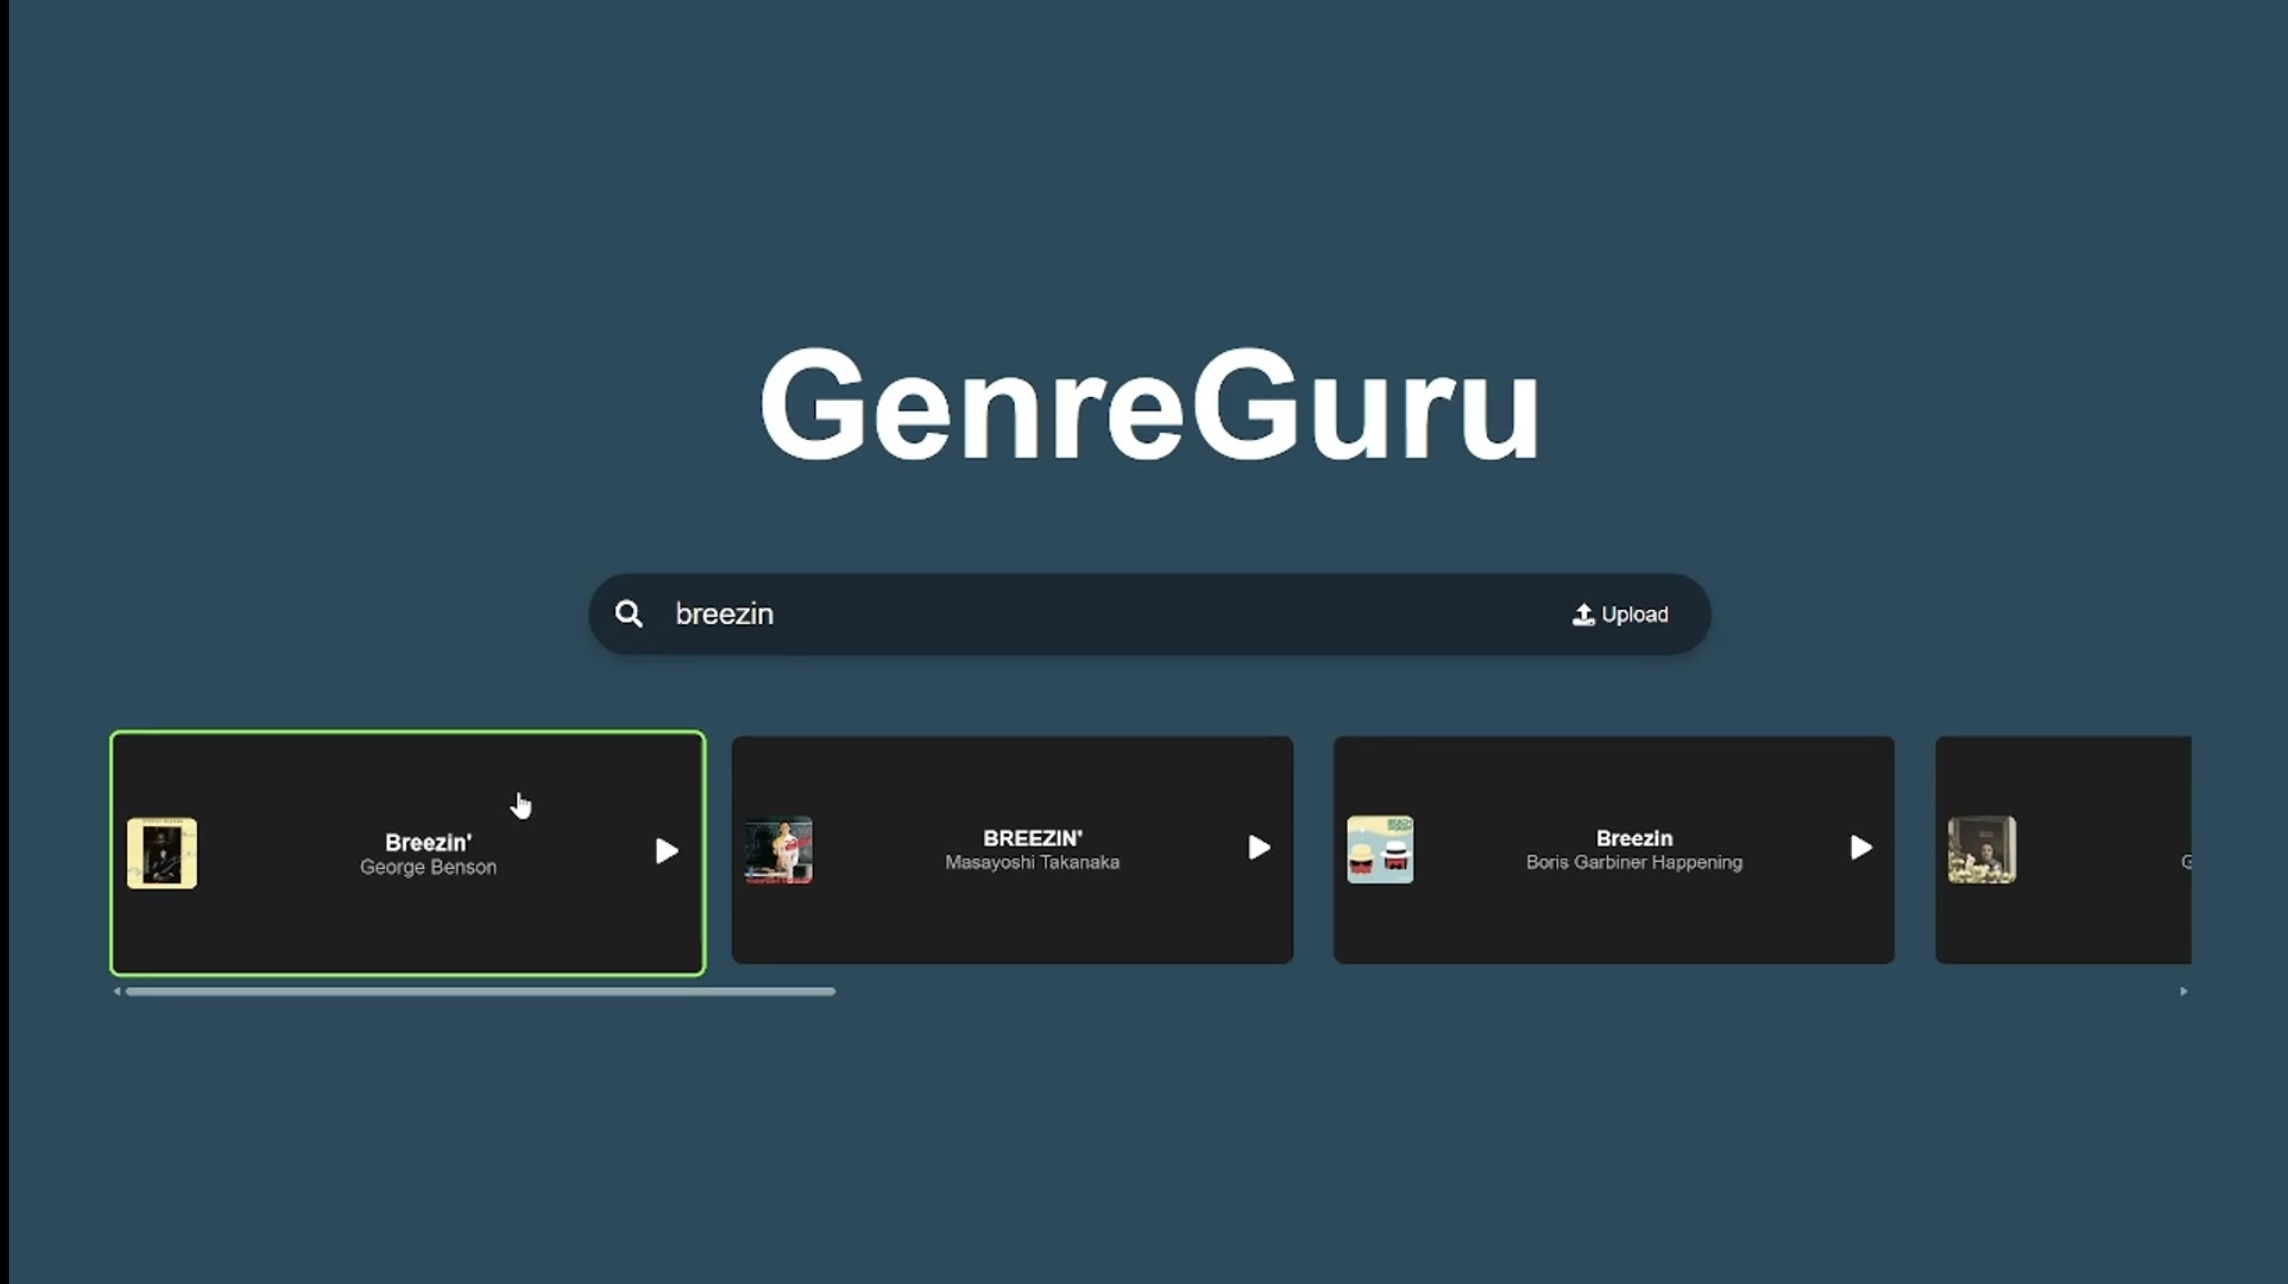
\includegraphics[width=\textwidth]{normans_principles_figures/img3.jpg}
    \caption{Track Selected with Visual Highlight}
    \label{img3}
\end{figure}

\begin{figure}[H]
    \centering
    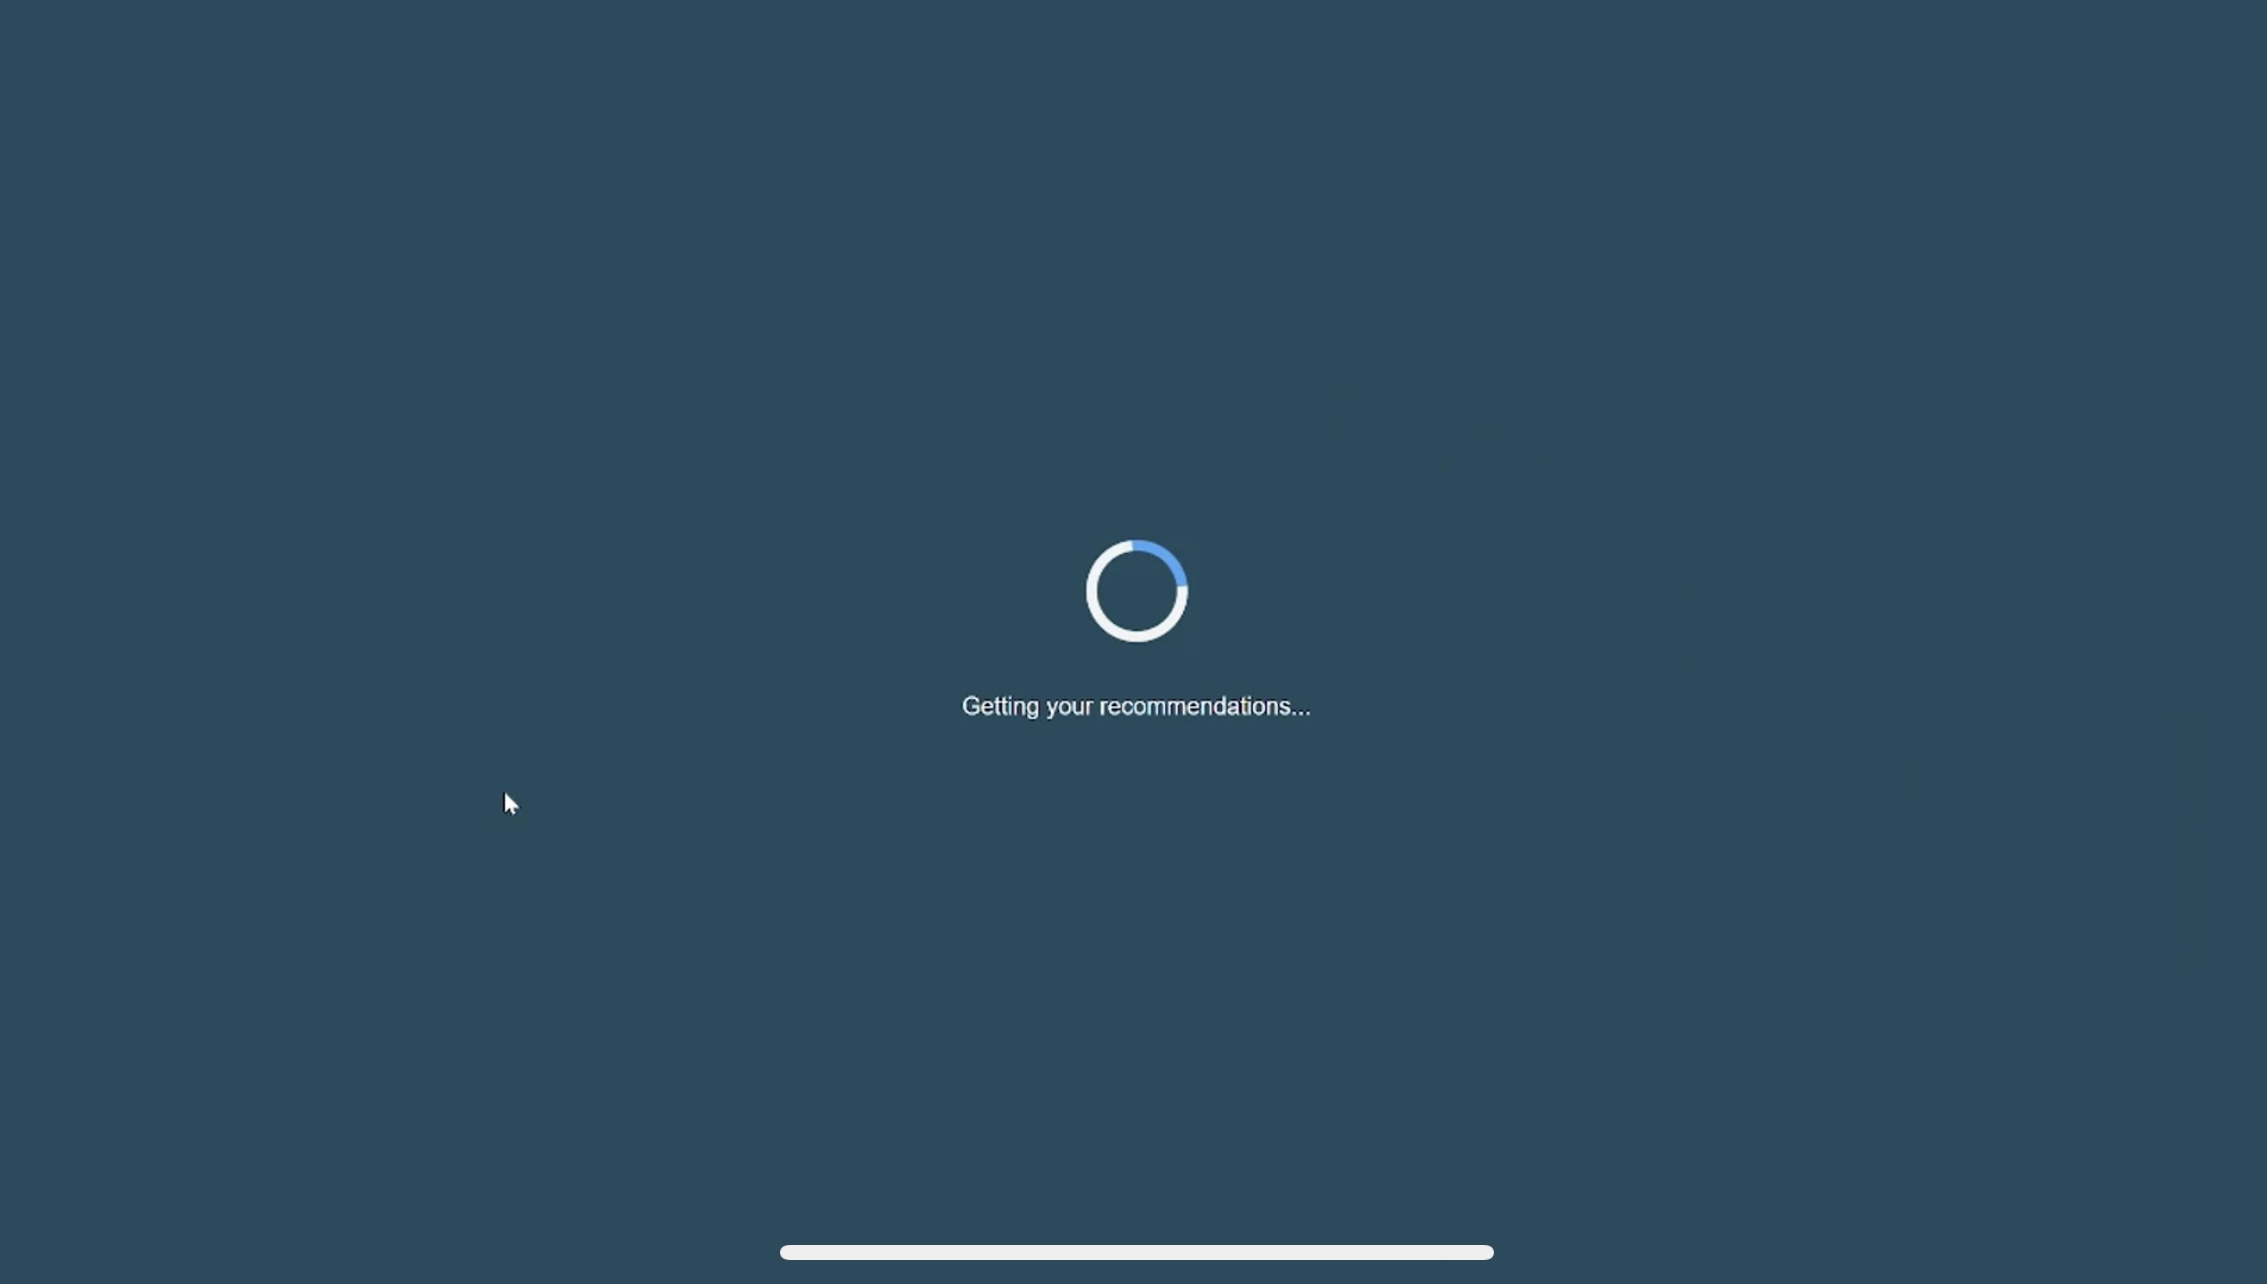
\includegraphics[width=\textwidth]{normans_principles_figures/img4.jpg}
    \caption{Loading Screen}
    \label{img4}
\end{figure}

\begin{figure}[H]
    \centering
    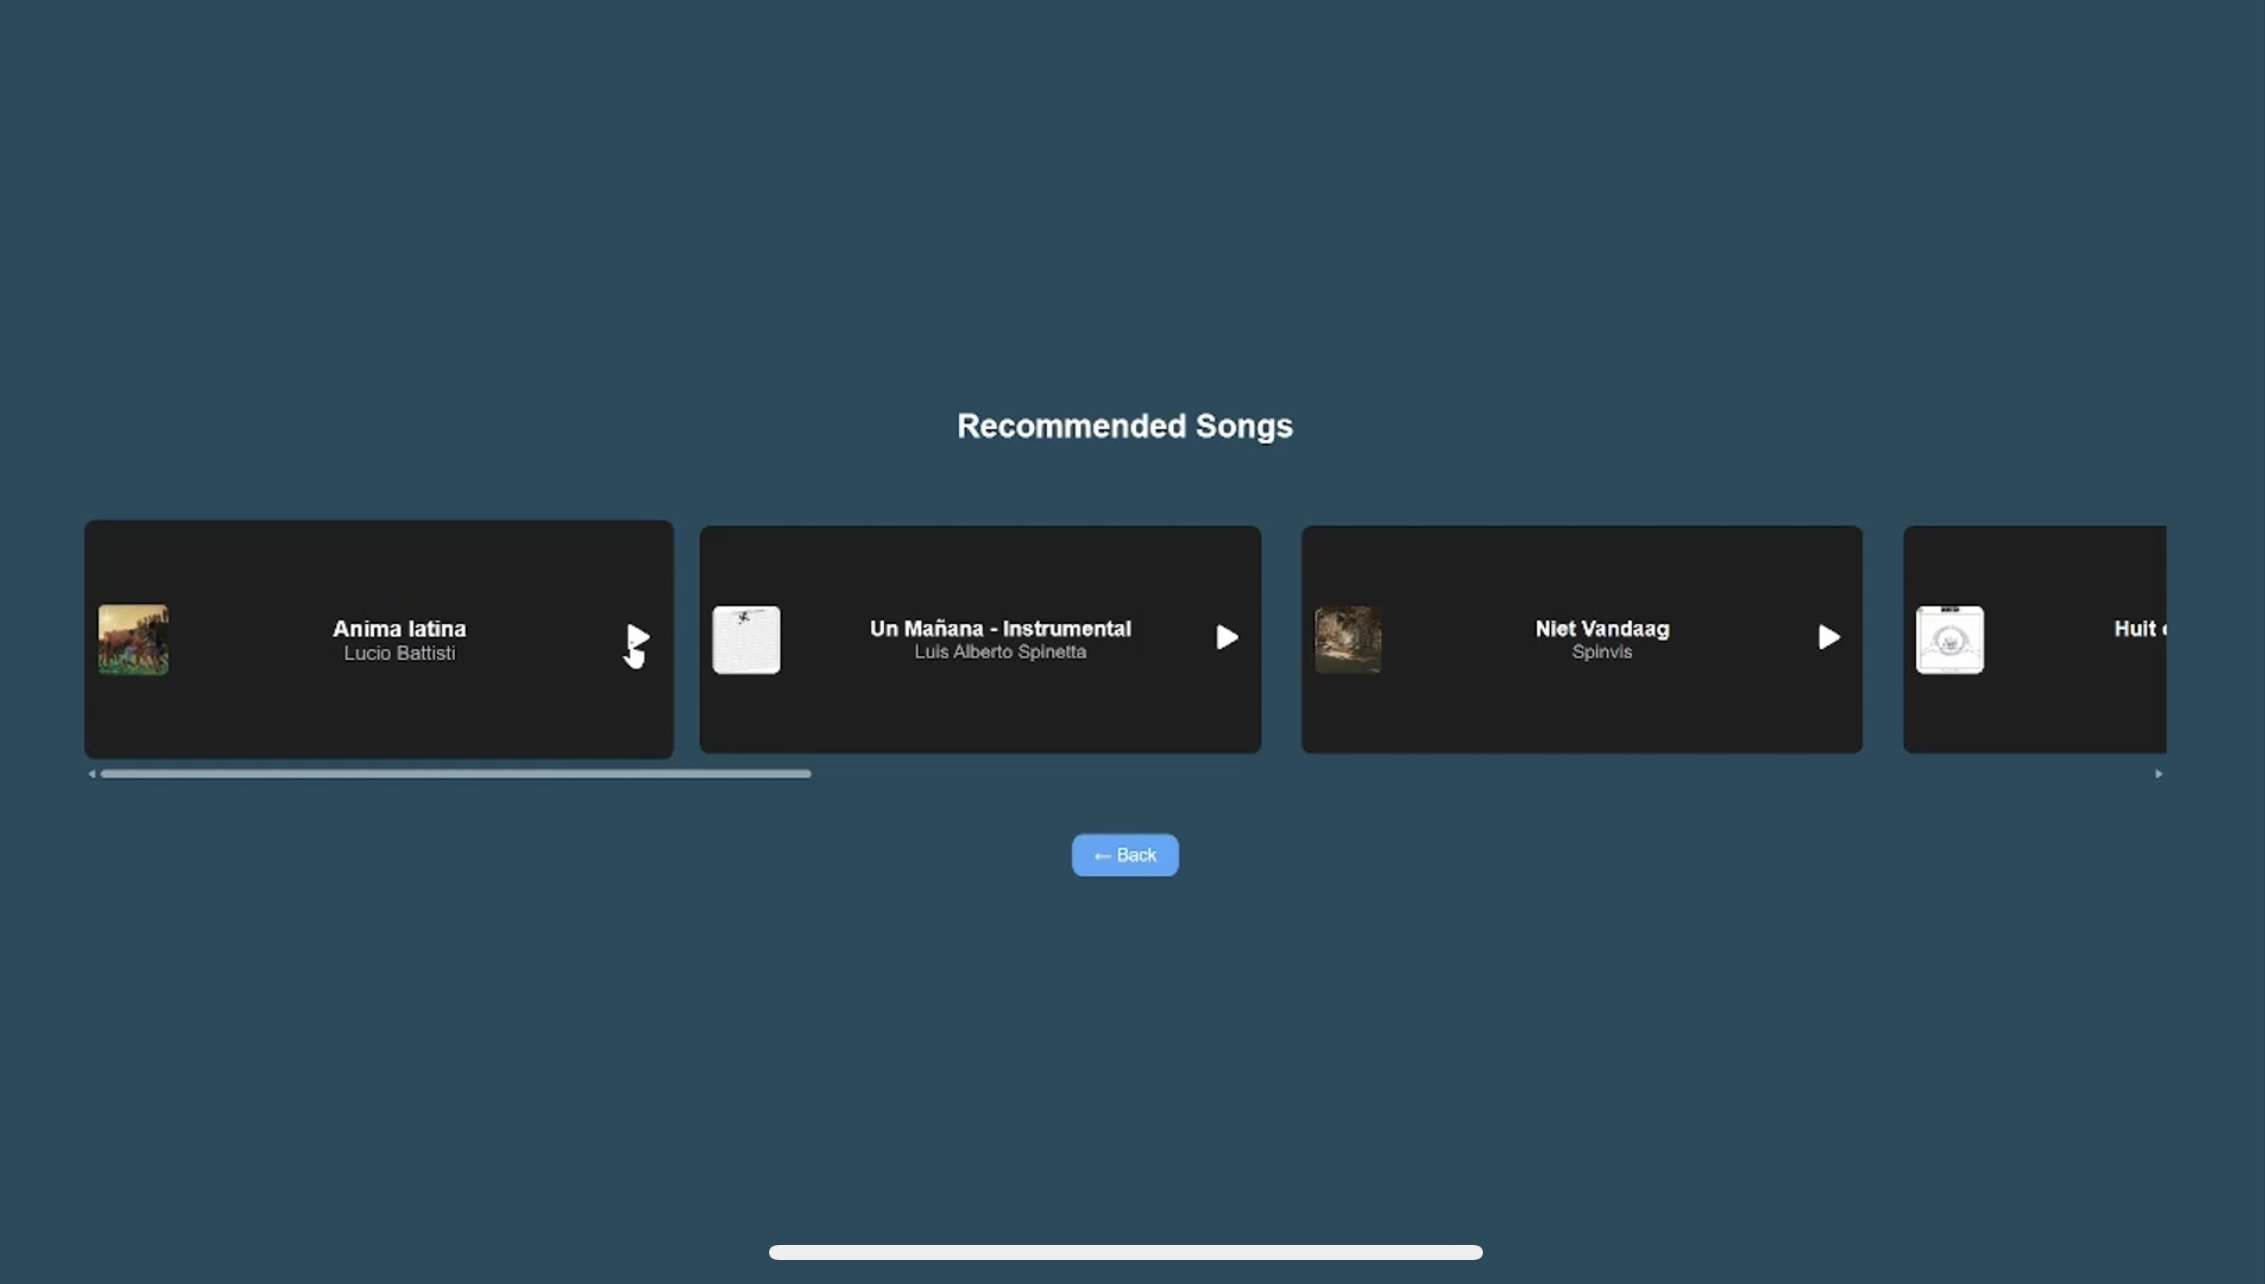
\includegraphics[width=\textwidth]{normans_principles_figures/img5.jpg}
    \caption{Recommendations Page}
    \label{img5}
\end{figure}

\section*{1. Visibility}

\noindent\textbf{Good:}
\begin{itemize}
    \item The search bar and upload button are immediately visible on the homepage (Figure~\ref{img1}). There is no clutter or ambiguity, and users instantly know where to begin.
    \item The "play" icons on search results and recommended tracks clearly show that previews are available (Figure~\ref{img2}, \ref{img5}).
    \item The track cards visibly display artist names and durations, enabling quick scanning by the user (Figure~\ref{img2}, \ref{img5}).
\end{itemize}

\noindent\textbf{Bad:}
\begin{itemize}
    \item When the system is loading, the feedback is textual but doesn’t communicate how long it might take or if progress is being made (Figure~\ref{img4}). A loading animation with an estimated time or progress indicator could help improve perceived responsiveness.
    \item The recommendation page lacks visibility on what action to take next (Figure~\ref{img5}). There is a "Back" button, but it's isolated and small, which may not be noticeable enough.
    \item There is no indication of a selected track on the recommendations screen, leaving users unclear whether the track has been successfully submitted.
\end{itemize}

\section*{2. Feedback}

\noindent\textbf{Good:}
\begin{itemize}
    \item When a user clicks a song, it is highlighted with a green border (Figure~\ref{img3}), visually indicating which track has been selected.
    \item A loading screen is presented after song selection (Figure~\ref{img4}), informing the user that the system is processing their request.
    \item The selected card changes its state upon being clicked (color highlight), giving real-time visual confirmation.
\end{itemize}

\noindent\textbf{Bad:}
\begin{itemize}
    \item Clicking the "Upload" button does not currently provide feedback (no modal or response is triggered as the feature is not working). Even for future fixes, an instant response (e.g. "file uploaded successfully") will be necessary.
    \item There is no feedback when a preview starts playing (no visual indication that audio is playing beyond sound).
    \item There is no hover state to indicate that icons (e.g., play, back) are interactive.
\end{itemize}

\section*{3. Affordance}

\noindent\textbf{Good:}
\begin{itemize}
    \item The magnifying glass icon next to the search bar clearly indicates that it is a search field (Figure~\ref{img1}).
    \item The play icon on each song tile invites the user to click and expect audio playback.
    \item The layout of song tiles resembles a media library, naturally inviting user interaction.
\end{itemize}

\noindent\textbf{Bad:}
\begin{itemize}
    \item The "Back" button appears clickable but lacks visual affordances like hover or click animations (Figure~\ref{img5}). It appears functional but feels static.
    \item Upload icon in the current implementation does not imply drag-and-drop or file select behavior, reducing the affordance for novice users.
    \item Search results do not provide tooltip guidance, such as “Click to play” or “Click to recommend,” which weakens intuitive interaction.
\end{itemize}

\section*{4. Mapping}

\noindent\textbf{Good:}
\begin{itemize}
    \item The linear, horizontal layout of search results and recommendations (Figure~\ref{img2} and \ref{img5}) maps well to expected behavior: scroll left to right to browse options.
    \item The position of the search bar in the center of the screen follows standard design conventions, mapping to what users expect when landing on a discovery platform.
    \item The play icon’s location on the right of the tile makes sense—consistent with common streaming platforms.
\end{itemize}

\noindent\textbf{Bad:}
\begin{itemize}
    \item The spacing between the Upload button and the search bar might confuse users who think both are part of the same action group, potentially making mapping less intuitive.
    \item Once results are displayed, it isn’t obvious whether clicking the card plays the preview or selects it for recommendation; users rely on trial and error.
    \item Clicking the tile vs. the play icon leads to different backend behavior, but this mapping is not visually communicated.
\end{itemize}


\section*{5. Constraints}

\noindent\textbf{Good:}
\begin{itemize}
    \item The interface constrains user actions nicely by limiting available paths: users can only either search or upload, and later, only select songs or go back.
    \item The "Search" input field limits to one input action and doesn’t allow multiple forms of user entry, helping reduce input complexity.
    \item Users cannot recommend a song unless a valid preview has been selected.
\end{itemize}

\noindent\textbf{Bad:}
\begin{itemize}
    \item On the search results page (Figure~\ref{img2}), it's possible to click multiple "play" icons in quick succession, resulting in overlapping previews.
    \item No input constraint on the search bar length or invalid characters handling is visible. There’s no warning for typos or empty search.
    \item There is no file format constraint indicator for the upload feature, even though only .wav files are currently processed.
\end{itemize}


\section*{6. Consistency}

\noindent\textbf{Good:}
\begin{itemize}
    \item Consistent font, color scheme, and button design throughout the system creates a professional and coherent visual language.
    \item Search and results pages use the same styling conventions, helping users stay oriented.
    \item All audio tiles follow a card-based layout, contributing to uniform visual expectations.
\end{itemize}

\noindent\textbf{Bad:}
\begin{itemize}
    \item The visual language of the "Back" button is inconsistent with the rest of the interface. It uses a different button style and breaks the visual rhythm.
    \item Preview icons are not consistently aligned across the cards, leading to slight visual irregularities (Figure~\ref{img2} and \ref{img5}).
    \item Button spacing is not uniform, especially between the "Upload" button and other controls, creating small usability inconsistencies.
\end{itemize}


\section*{Conclusion}
The final UI design of GenreGuru aligns well with Norman's principles in many respects. Visibility and feedback are strong in the main flows of the application, particularly around search and track selection. However, there is room for improvement in areas like feedback during audio playback, upload affordance, and consistency of button styles.

Our retrospective evaluation revealed valuable opportunities to tighten design cohesion and enhance intuitiveness. We believe that by improving these targeted areas, GenreGuru can deliver an even more polished and user-friendly experience.


\end{document}
